\documentclass[]{exam}
\usepackage{epic,array,ecltree,url,calrsfs}
\usepackage[nointegrals]{wasysym}

%These tell TeX which packages to use.
\usepackage{array,epsfig}
\usepackage{amsmath}
\usepackage{amsfonts}
\usepackage{amssymb}
\usepackage{amsxtra}
\usepackage{amsthm}
\usepackage{mlextra} % must come after ams packages
\usepackage{mathrsfs}
\usepackage[dvipsnames]{xcolor}
\usepackage{array}
\usepackage{graphicx}
\graphicspath{ {../art/} }
\usepackage{bm}
\usepackage{tikz}
\usepackage{multicol}
\usepackage{enumitem}

\newcommand{\twonode}{%
  \begingroup\normalfont
  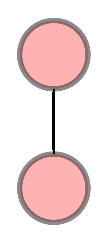
\includegraphics[height=\fontcharht\font`\b]{2nodetree.eps}%
  \endgroup
}

\newcommand{\tf}[1][{}]{%
\fillin[#1][0.25in]%
}
\title{Lab 7: Complexity, DPLL, FOL Basics}
\author{Foundations of Computer Science}
\date{\today}
%\pagestyle{empty} 
%\footer{}{\thepage}{}
\noprintanswers
\unframedsolutions
\SolutionEmphasis{\itshape\small}
\SolutionEmphasis{\color{NavyBlue}}


\begin{document}

\maketitle
\setlength{\columnseprule}{1pt}
\section*{Complexity}
\begin{questions} 
\question If a problem $A$ is in $\id{NP}$, its complement is in \fillin[CoNP].
\question We say $A$ is $\id{NP}$-Hard iff it is \fillin all problems in $\id{NP}$.
\begin{checkboxes}
\choice harder than
\choice as hard as
\CorrectChoice at least as hard as
\choice no harder than
\end{checkboxes}

\question \tf[F] (T/F) If $A$ is $\id{NP}$-Hard, $A$ is in $\id{NP}$.
\question \tf[T] (T/F) If $A$ is $\id{NP}$-Complete, $A$ is in $\id{NP}$.
\question \tf[T] (T/F) If $A$ is $\id{NP}$-Complete, $A$ is $\id{NP}$-Hard.

\question Let $A$ and $B$ be problems such that $A$ is $\id{NP}$-Complete
and $A$ reduces to $B$. What can we say about $B$?
\begin{checkboxes}
\choice It is smaller than $A$.
\choice It is harder than $A$.
\CorrectChoice It is at least as hard as $A$.
\CorrectChoice It is $\id{NP}$-Hard.
\end{checkboxes}

\section*{DPLL}

\question Let $S$ be a formula of propositional logic in clausal form such that
$S = \{pqr, \bar{p}q, \bar{q}\bar{r}, r \}$\\

\begin{parts}
\part\label{q:dpllpT} Assume $p$ is $T$, and produce an equisatisfiable formula under this
assumption.
\begin{solution}
$\{q, \bar{q}\bar{r}, r \}$
\end{solution}

\part Repeat part (\ref{q:dpllpT}) but assume $p$ is $F$.
\begin{solution}
$S = \{qr, \bar{q}\bar{r}, r \}$\\
\end{solution}

\end{parts}

\question Use DPLL to refute the following formula from Lab 6: $\{p, \bar{p}qr, \bar{p}\bar{q}\bar{r}, \bar{p}st, \bar{p}\bar{s}\bar{t}, \bar{s}q, rt, \bar{t}s\}$\\
Draw the recursive execution tree. 
\begin{solution}
\begin{center}
\begin{picture}(200,160)
\put(100,160){
  \put( -10,   0){\makebox(20,10){$\{p, \bar{p}qr, \bar{p}\bar{q}\bar{r}, \bar{p}st, \bar{p}\bar{s}\bar{t}, \bar{s}q, rt, \bar{t}s\}$}}
  \put( -60, -17){\makebox(20,10){$p$}}
  \put(  45, -17){\makebox(20,10){$\bar{p}$}}
  \put( -85, -35){\makebox(20,10){$\{qr, \bar{q}\bar{r}, st, \bar{s}\bar{t}, \bar{s}q, rt, \bar{t}s\}$}}
  \put(  65, -35){\makebox(20,10){$\{\Box, \bar{s}q, rt, \bar{t}s\}$}}
  \put(-122, -55){\makebox(20,10){$s$}}
  \put(- 42, -55){\makebox(20,10){$\bar{s}$}}
  \put(-142, -76){\makebox(20,10){$\{qr, \bar{q}\bar{r}, \bar{t}, q, rt \}$}}
  \put( -22, -76){\makebox(20,10){$\{qr, \bar{q}\bar{r}, t, rt, \bar{t}\,\}$}}
% \put(  65, -76){\makebox(20,10){true}}
  \put(- 42, -90){\makebox(20,10){$t$}}
  \put(   3, -90){\makebox(20,10){$\bar{t}$}}
  \put(-167, -90){\makebox(20,10){$q$}}
  \put(-122, -90){\makebox(20,10){$\bar{q}$}}
  \put(-175,-108){\makebox(20,10){$\{\bar{r}, \bar{t}, rt \}$}}
  \put(-110,-108){\makebox(20,10){$\{r, \bar{t}, \Box, rt \}$}}
  \put(- 50,-108){\makebox(20,10){$\{qr, \bar{q}\bar{r}, \Box \}$}}
  \put(  15,-108){\makebox(20,10){$\{qr, \bar{q}\bar{r}, \Box, r \}$}}
  \put(-203,-122){\makebox(20,10){$r$}}
  \put(-155,-122){\makebox(20,10){$\bar{r}$}}
  \put(-212,-140){\makebox(20,10){$\{\Box, \bar{t} \}$}}
  \put(-150,-140){\makebox(20,10){$\{\bar{t}, t \}$}}
  \put(-165,-153){\makebox(20,10){$t$}}
  \put(-135,-153){\makebox(20,10){$\bar{t}$}}
  \put(-170,-170){\makebox(20,10){$\{\Box, \Box \}$}}
  \put(-130,-170){\makebox(20,10){$\{\Box, \Box \}$}}
  \put(   0,   0){\line(-3,-1){68}}
  \put(   0,   0){\line( 3,-1){68}}
  \put( -74, -35){\line(-2,-1){58}}
  \put( -74, -35){\line( 2,-1){58}}
% \put(  75, -35){\line(0,-1){28}}
  \put(-135, -76){\line(-3,-2){30}}
  \put(-135, -76){\line( 3,-2){30}}
  \put(- 10, -76){\line(-3,-2){30}}
  \put(- 10, -76){\line( 3,-2){30}}
  \put(-170,-108){\line(-3,-2){30}}
  \put(-170,-108){\line( 3,-2){30}}
  \put(-140,-140){\line(-1,-1){18}}
  \put(-140,-140){\line( 1,-1){18}}
}
\end{picture}
\end{center}


\end{solution}
\question Let $A$ be the formula $(r \imp s) \land (s \imp \ngg t) \land (\ngg r \imp \ngg t)$.
Use DPLL to determine whether $A$ is a contradiction. If it is not, give an
interpretation that satisfies $A$.
\begin{solution}
~\\
First, change to clausal form: $\{\bar{r}s,\bar{s}\bar{t},r\bar{t}\}$\\
Then eliminate $\bar{t}$, since it only appears with one polarity, to get: $\{\bar{r}s,\bar{s},r\}$\\
Unit propagation on $r$ gives: $\{s,\bar{s}\}$\\
Unit propagation on $s$ gives: $\{\}$\\
Therefore, the formula is satisfiable. Tracing back the steps, we have
$v_{\mathcal{I}_A}(s) = T, v_{\mathcal{I}_A}(r) = T$ and $v_{\mathcal{I}_A}(r)$
can be true or false.
\end{solution}

\question Let $p_{ij}$ represent the statement ``pidgeon number $i$ is in hole number $j$.''
\begin{parts}
\part Give an informal summary of the following statement:\\ 
$(p_{11} \lor p_{12} \lor p_{13}) \land  
 (p_{21} \lor p_{22} \lor p_{23}) \land  
 (p_{31} \lor p_{32} \lor p_{33}) \land  
 (p_{41} \lor p_{42} \lor p_{43})$
\begin{solution}
Pidgeons $1,2,3$ and $4$ are in holes $1,2$ or $3$.
\end{solution}

\part Give an informal summary of the following statement:\\
$\ngg (p_{11} \land p_{21}) \land
 \ngg (p_{11} \land p_{31}) \land
 \ngg (p_{11} \land p_{41}) \land
 \ngg (p_{21} \land p_{31}) \land
 \ngg (p_{21} \land p_{41}) \land
 \ngg (p_{31} \land p_{41})$
\begin{solution}
Only one of the pidgeons $1,2,3$ and $4$ is in hole $1$.
\end{solution}


\part Build on the statements above to express the pidgeon-hole problem for the
      case where there are $3$ holes and $4$ pigeons.
\begin{solution}
~\\
$(p_{11} \lor p_{12} \lor p_{13}) \land  
 (p_{21} \lor p_{22} \lor p_{23}) \land  
 (p_{31} \lor p_{32} \lor p_{33}) \land  
 (p_{41} \lor p_{42} \lor p_{43}) \land $\\
$\ngg (p_{11} \land p_{21}) \land
 \ngg (p_{11} \land p_{31}) \land
 \ngg (p_{11} \land p_{41}) \land
 \ngg (p_{21} \land p_{31}) \land
 \ngg (p_{21} \land p_{41}) \land
 \ngg (p_{31} \land p_{41}) \land$ \\
$\ngg (p_{12} \land p_{22}) \land
 \ngg (p_{12} \land p_{32}) \land
 \ngg (p_{12} \land p_{42}) \land
 \ngg (p_{22} \land p_{32}) \land
 \ngg (p_{22} \land p_{42}) \land
 \ngg (p_{32} \land p_{42}) \land$ \\
$\ngg (p_{13} \land p_{23}) \land
 \ngg (p_{13} \land p_{33}) \land
 \ngg (p_{13} \land p_{43}) \land
 \ngg (p_{23} \land p_{33}) \land
 \ngg (p_{23} \land p_{43}) \land
 \ngg (p_{33} \land p_{43}) $
 
 \end{solution}


\part Change your statement to clausal form.
\begin{solution}
~\\
$\{p_{11}p_{12}p_{13}, 
   p_{21}p_{22}p_{23}, 
   p_{31}p_{32}p_{33}, 
   p_{41}p_{42}p_{43},
 \bar{p_{11}}\bar{p_{21}},
 \bar{p_{11}}\bar{p_{31}},
 \bar{p_{11}}\bar{p_{41}},
 \bar{p_{21}}\bar{p_{31}},
 \bar{p_{21}}\bar{p_{41}},
 \bar{p_{31}}\bar{p_{41}},$ \\
$\bar{p_{12}}\bar{p_{22}},
 \bar{p_{12}}\bar{p_{32}},
 \bar{p_{12}}\bar{p_{42}},
 \bar{p_{22}}\bar{p_{32}},
 \bar{p_{22}}\bar{p_{42}},
 \bar{p_{32}}\bar{p_{42}},
 \bar{p_{13}}\bar{p_{23}},
 \bar{p_{13}}\bar{p_{33}},
 \bar{p_{13}}\bar{p_{43}},
 \bar{p_{23}}\bar{p_{33}},
 \bar{p_{23}}\bar{p_{43}},
 \bar{p_{33}}\bar{p_{43}}\}$ 
 \end{solution}


\part Use DPLL to show the statement is unsatisfiable for \emph{one} assignment.
\begin{solution}
~\\Checking one assignment is equivalent to only taking one branch at each split.
\begin{enumerate}
\item Begin with $v(p_{11}) = T$. The equisatisfiable clause under this case is:\\
$\{ 
   p_{21}p_{22}p_{23}, 
   p_{31}p_{32}p_{33}, 
   p_{41}p_{42}p_{43},$ \\
$            \bar{p_{21}},
             \bar{p_{31}},
             \bar{p_{41}},
 \bar{p_{21}}\bar{p_{31}},
 \bar{p_{21}}\bar{p_{41}},
 \bar{p_{31}}\bar{p_{41}},$ \\
$\bar{p_{12}}\bar{p_{22}},
 \bar{p_{12}}\bar{p_{32}},
 \bar{p_{12}}\bar{p_{42}},
 \bar{p_{22}}\bar{p_{32}},
 \bar{p_{22}}\bar{p_{42}},
 \bar{p_{32}}\bar{p_{42}},
 \bar{p_{13}}\bar{p_{23}},$ \\
$\bar{p_{13}}\bar{p_{33}},
 \bar{p_{13}}\bar{p_{43}},
 \bar{p_{23}}\bar{p_{33}},
 \bar{p_{23}}\bar{p_{43}},
 \bar{p_{33}}\bar{p_{43}}\}$ \\
\item This leaves unit clauses $\bar{p_{21}}, \bar{p_{31}}, \bar{p_{41}}$. Performing
unit propagation on these leaves:\\
$\{ 
         p_{22}p_{23}, 
         p_{32}p_{33}, 
         p_{42}p_{43},$ \\
$\bar{p_{12}}\bar{p_{22}},
 \bar{p_{12}}\bar{p_{32}},
 \bar{p_{12}}\bar{p_{42}},
 \bar{p_{22}}\bar{p_{32}},
 \bar{p_{22}}\bar{p_{42}},
 \bar{p_{32}}\bar{p_{42}},$\\
$\bar{p_{13}}\bar{p_{23}},
 \bar{p_{13}}\bar{p_{33}},
 \bar{p_{13}}\bar{p_{43}},
 \bar{p_{23}}\bar{p_{33}},
 \bar{p_{23}}\bar{p_{43}},
 \bar{p_{33}}\bar{p_{43}}\}$ \\

\item Next assign $v(p_{22}) = T$. This leads to the following clause:\\
$\{ 
         p_{32}p_{33}, 
         p_{42}p_{43},$ \\
$\bar{p_{12}},
 \bar{p_{12}}\bar{p_{32}},
 \bar{p_{12}}\bar{p_{42}},
             \bar{p_{32}},
             \bar{p_{42}},
 \bar{p_{32}}\bar{p_{42}},$\\
$\bar{p_{13}}\bar{p_{23}},
 \bar{p_{13}}\bar{p_{33}},
 \bar{p_{13}}\bar{p_{43}},
 \bar{p_{23}}\bar{p_{33}},
 \bar{p_{23}}\bar{p_{43}},
 \bar{p_{33}}\bar{p_{43}}\}$ \\
\item Next perform unit propagation again on $\bar{p_{12}}, \bar{p_{32}}$ and
$\bar{p_{42}}$ to get:\\
$\{ 
               p_{33}, 
               p_{43},
 \bar{p_{13}}\bar{p_{23}},
 \bar{p_{13}}\bar{p_{33}},
 \bar{p_{13}}\bar{p_{43}},
 \bar{p_{23}}\bar{p_{33}},
 \bar{p_{23}}\bar{p_{43}},
 \bar{p_{33}}\bar{p_{43}}\}$ \\
\item Finally, unit propagation on $p_{33}$ and $p_{43}$ produce:\\
$\{ 
               p_{43},
 \bar{p_{13}}\bar{p_{23}},
 \bar{p_{13}}            ,
 \bar{p_{13}}            ,
 \bar{p_{23}}            ,
 \bar{p_{23}}            ,
             \Box       \}$ \\
\end{enumerate}
\end{solution}
\end{parts}
\section*{First Order Logic}
\question Write an informal statement of the following formula under the
interpretations given below:\\ 
$\forall x \exists y (p(x,a) \imp (p(y,a) \land p(x,y)))$
\begin{parts}
\part $(\N_0,\{>\},\{0\})$
\begin{solution}
Every natural number greater than $0$ is also greater than some other
natural number that it greater than $0$.
\end{solution}

\part $(\N_0,\{\geq \},\{0\})$
\begin{solution}
Every natural number greater than or equal to $0$ is also greater than or
equal to some other natural number that is greater than or equal to $0$.
\end{solution}

\part $(\{0,1,2\},\{\neq\},\{0\})$
\begin{solution}
Out of the three numbers $0,1$ and $2$, either of the two numbers that
is not equal to zero is also not equal to some other nonzero number in the 
set.
\end{solution}

\end{parts}
\question Repeat the exercise above with the following formula and the
interpretations listed below: \\
$\forall x \forall y (p(x,y) \imp \exists z (p(x,z) \land p(z,y)))$
\begin{parts}
\part $(\Q,\{<\},\{\})$
\begin{solution}
There is a rational number between any two rational numbers.
\end{solution}

\part $(\Z,\{<\},\{\})$
\begin{solution}
There is an integer between any two integers.
\end{solution}

\part $(\{a,b\}^*, \{substr\},\{\})$ (where $substr$ is a binary relation such
    that $(s_1,s_2) \in substr$ iff $s_1$ is a substring of $s_2$).
\begin{solution}
For any two strings $s_1$ and $s_2$ where $s_1$ is a substring of $s_2$, there
is always a string $s_3$ such that $s_1$ is a substring of $s_3$ and $s_3$ is 
a substring of $s_2$.
\end{solution}

\end{parts}

% Next year: give a policy statement and ask students to write it in FOL
% Everyone in the Navy can read the document.
% The author can delete it.
% Anyone in the class can edit it.
% A

\end{questions}
\end{document}


